\documentclass[a4paper]{article}

\usepackage{geometry}
\usepackage{natbib}
\bibpunct[:]{(}{)}{,}{a}{}{;}

%--------------------
%\usepackage{gb4e}
%\noautomath

\usepackage{amsmath}
\usepackage{amsfonts}
\usepackage{amsthm}
\usepackage{amssymb}
\usepackage{mathrsfs}
\usepackage{nicefrac}
%\usepackage{stmaryrd}
%\usepackage{multicol}
\usepackage{graphicx}
\usepackage{color}
%\newcommand{\mvalueof}[1]{\llbracket#1\rrbracket}
\newcommand{\citeposs}[2][]{\citeauthor{#2}'s (\citeyear[#1]{#2})}
\newcommand{\tuple}[1]{\ensuremath{\left\langle #1 \right\rangle}} 

\newcommand{\hl}[1]{\textcolor[rgb]{.8,.33,.0}{#1}}% prints in orange
%\newcommand{\argmax}[1]{\underset{#1}{\operatorname{arg}\,\operatorname{max}}\;}
%\newcommand{\argmin}[1]{\underset{#1}{\operatorname{arg}\,\operatorname{min}}\;}
%\newcommand{\sbna}{\exists\lnot\forall}

%--------------------
%
%\usepackage{setspace}
%\onehalfspacing
%
%-------------------


\title{Communicative pressures at the semantics-pragmatics interface:\\ Learning biases may prevent the lexicalization of pragmatic inferences}

\author{%\bf NAME1 and NAME2\\
    ( -- draft \today --- )
}


\date{}

\begin{document}
\maketitle

\begin{abstract} Certain lexical meanings enable for pragmatic enrichments in a notably productive fashion. This raises the challenge to justify their regular selection, in particular, over alternatives that codify semantically what is conveyed pragmatically. To address this challenge, we propose a general model that integrates iterated Bayesian learning in the replicator-mutator dynamics. This model allows for population-level analyses of the effects of linguistic pressures on probabilistic language users with varied degrees of pragmatic sophistication and distinct languages. We showcase the model's use and predictions in a case study on the (lack of) lexicalization of scalar implicatures. The results suggest simpler semantic representations to be selected for when languages are pressured towards learnability and compression, provided that pragmatic reasoning can compensate for the disadvantage in expressivity that users of such languages otherwise incur.


\section{The semantics-pragmatics divide}\label{sec:introduction}

\end{abstract}

In linguistic theorizing, it is common to draw a distinction between semantics and pragmatics. Broadly speaking, the former concerns the truth-conditional content of expressions, whereas the latter concerns information beyond literal meanings and their composition. An important consequence of this distinction is that the information conveyed by an utterance is seldom, if ever, solely determined by semantics, but rather in tandem with pragmatics. 

Much research at the semantics-pragmatics interface has been aimed at characterizing expressions in terms of either domain, or their interplay. However, an issue that has received little attention is the justification of semantic structure in light of pragmatics. The present investigation seeks to fill this gap by analyzing the effects linguistic pressures have on the selection and pervasiveness of particular lexical meanings under consideration of pragmatic enrichments.

In recent years, similar questions about the emergence and change of linguistic features have lead to a surge in models to address them (see \citealt{steels:2015} and \citealt{tamariz+kirby:2016} for recent overviews). Our starting point is given by the overarching argument that has crystalized from accumulated mathematical, experimental and cross-linguistic evidence in this literature: Natural languages need to be well-adapted to communicative needs within a linguistic community, but also need to be learnable to survive their faithful transmission across generations. More succinctly; natural languages are pressured for expressiveness as well as learnability.   

We build on these insights by modeling these pressures using the replicator-mutator dynamics (see \citealt{hofbauer+sigmund:2003} for an overview). This allows for the inspection of their interaction by combining functional pressure on successful communication with effects of learning biases on (iterated) Bayesian learning \citep{griffiths+kalish:2007}. The semantics-pragmatics distinction and its effect on production and comprehension is made precise by considering probabilistic models of rational language use in populations with distinct lexica \citep{frank+goodman:2012,franke+jaeger:2014, bergen+etal:2016}. 

%In this way, the model establishes a link between models of synchronic probabilistic rational language use and diachronic models of cultural evolution. 

%We then analyze the prevalence of a lack of semantic upper-bounds in the literal meaning of weak scalar expressions. We show that a lack of upper-bounds is selected for when learners are biased towards simpler semantic representations, provided they have means to convey upper-bounds, i.e., provided that they can be derived via pragmatic reasoning.  


\section{Simplicity, expressivity, and learnability}

The emergence and change of linguistic structure is influenced by many intertwined factors, ranging from biological and socio-ecological to cultural \citep{steels:2011,tamariz+kirby:2016}. Social and ecological pressures determine communicative needs, while biology determines the architecture that enables and constrains their means of fulfillment. In the following, our focus lies on the latter, cultural factor, wherein processes of linguistic change are understood as shaped by its use and transmission. That is, as a result of cultural evolution.

At latest since \citeposs{zipf:1949} rationalization of the observation that word frequency rankings can be approximated by a power law distribution as competing hearer and speaker preferences, the idea that linguistic change is influenced by communicative pressures has played a pivotal role in synchronic and diachronic analyses (e.g. \citealt{martinet:1962, horn:1984,jaeger+vRooij:2007,jaeger:2007, piantadosi:2014,kirby+etal:2015}). 

As noted above, expressivity and learnability are two major competing pressures. Their opposition becomes particularly clear when considering their consequences in the extreme (cf. \citealt{kemp+regier:2012,kirby+etal:2015}). On the one side, a language with a single form is easy to learn but lacking in expressivity for most purposes. On the other, a language that associates a distinct form with all possible meanings its users may want to convey is maximally expressive but challenging to acquire. The most prominent problem that arises from this tension is that of acquiring a language to express a potentially infinite set of meanings through finite means \citep{kirby:2002}. However, this so-called transmission bottleneck is not the only challenge learners confront. 

More important for our purposes is the problem of selecting particular hypotheses out of a potentially infinite space of alternatives compatible with the data learners are exposed to. At the semantics-pragmatics interface this concerns the selection between functionally similar, if not identical, lexical meanings.  In the following, we argue an integral part of the answer to be that learners are a priori biased towards simpler, more compressed, lexical representations. This corresponds to the argument that rational learners should prefer simpler over more complex explanations of data \citep{feldman:2000, chater+vitanyi:2003, piantadosi+etal:2012a, kirby+etal:2015,piantadosi+etal:underreview}. In linguistics, a drive for simplicity has been argued to underpin speaker preferences for brevity and ease of articulation, as well as to pressure languages towards lexical ambiguity and grammatical compression \citep{zipf:1949,grice:1975,piantadosi+etal:2012, kirby+etal:2015}. As a broader cognitive principle, the use of simplicity as means to select between hypotheses has a long standing tradition. Crucially, \citet{chater+vitanyi:2003} give a number of compelling arguments for simplicity on both mathematical and empirical grounds.


The remainder of this section introduces the individual components of the model in more detail, as well as the assumptions underlying them. These are: (i) languages and their use, (ii) pressures towards expressivity and learnability, regulated by the replicator and mutator dynamics, respectively, as well as (iii) a bias towards simpler semantic representations, codified as a language learner's prior. After laying out the model, we discuss its application to the lack of lexicalization of scalar implicatures.



%The observation that monomorphemic expression that lexically rule out stronger alternatives (e.g. {not all} as hypothetical `nall') are unattested across languages has received substantial argumentative support (most prominently in \citealt[252-267]{horn:1984} but also e.g. in \citealt{horn:1972,traugott:2004,vdAuwera:2010}). To the best of our knowledge, this claim stands unchallenged.

\subsection{Languages and linguistic behavior}
Lexica codify the truth-conditions of a language's expressions, i.e., its semantics. A convenient way to represent such lexica is by $(|S|,|M|)$-Boolean matrices, where $S$ is a set of states of affairs, or meanings, to convey and $M$ a set of messages of the language \citep{franke+jaeger:2014}. For instance, the following two lexica fragments determine the truth-conditions of two messages, $m_1$ and $m_2$, for two states, $s_1$ and $s_2$:

\begin{centering}
$L_a$ = \bordermatrix{~ & m_1 & m_2 \cr 
                  s_1 & 1 & 0 \cr
                  s_2 & 1 & 1 \cr} \hspace{2cm} $L_b$ = \bordermatrix{~ & m_1 & m_2 \cr 
                  s_1 & 1 & 0 \cr
                  s_2 & 0 & 1 \cr}\\[0.5cm]
\end{centering}


In words, according to lexicon $L_a$, $m_1$ is true of state $s_1$ as well as of $s_2$. In contrast, message $m_1$ is only true of $s_1$ in $L_b$. Otherwise, the two languages are truth-conditionally equivalent. 

To make the distinction betweeen semantics and pragmatics precise, we distinguish between two kinds of linguistic behavior. {\em Literal interlocutors} produce and interpret messages literally. That is, their linguistic choices are guided by their lexica only. In contrast, {\em pragmatic interlocutors} engage in mutual reasoning to inform their choices. For instance, a rational speaker of $L_a$ who reasons about her addressee should use $m_1$ to signal state $s_1$ given that $m_2$ is already unambiguously associated with state $s_2$. Analogously, should rational hearers expect their interlocutors to reason along these lines, they will interpret ambiguous $m_1$ accordingly. Note in particular that according to this strenghtening of $m_1$, $L_a$ is indistinguishable from $L_b$ in terms of expressiveness if its users are pragmatic reasoners.

Following models of rational language use such as Rational Speech Act models \citep{frank+goodman:2012} and their game-theoretic counterparts \citep{benz+etal:2005a,franke:2009,franke+jaeger:2014}, this kind of signaling behavior is captured by a hierarchy over reasoning types. The hierarchy's bottom, level $0$, corresponds to literal language use. Pragmatic language users of level $n + 1$ behave rationally according to (expected) level $n$ behavior of their interlocutors. The behavior of literal and pragmatic hearers of a language $L$ is given by their respective selection functions in (\ref{h:level0}) and (\ref{h:leveln}). Mutatis mutandis for the speaker functions in (\ref{s:level0}) and (\ref{s:leveln}).

\begin{flalign}
&H_{0}(s|m;L) \propto pr(s) L_{sm} \label{h:level0}\\
&S_{0}(m|s;L) \propto \exp(\lambda \; L_{sm}) \label{s:level0}\\
&H_{n+1}(s|m;L) \propto pr(s) S_{n}(m|s;L) \label{h:leveln}\\
&S_{n+1}(m|s;L) \propto  \exp(\lambda \; H_{n}(s|m;L)^\alpha) \label{s:leveln}
\end{flalign}

According to (\ref{h:level0}), a literal hearer's interpretation of a message $m$ as a state $s$ depends on her lexicon and her prior over states, $pr \in \Delta(S)$. The literal speaker's choice in (\ref{s:level0}) is regulated by a soft-max parameter $\lambda$, $\lambda \geq 1$ \citep{luce:1959,sutton+barto:1998}. As $\lambda$ increases, choices made in production are more rational in that higher values lead to more deterministic in line with expected utility maximization.

For the most part, pragmatic behavior mirrors its literal counterpart. As described above, their difference lies in that level $n+1$ speakers/hearers reason about level $n$ hearer/speaker behavior instead of solely relaying on their lexicon. That is, they reason about how a rational level $n$ interlocutor would use or interpret a message and behave according to these expectations. Additionally, pragmatic production is further regulated by a parameter $\alpha$ which controls the tension between semantics and pragmatics, $\alpha \in (0,1]$. Lower values lead to more literal production, whereas higher values lead to stronger pragmatic behavior. 

The combination of a lexicon with its use, i.e., a particular level of linguistic sophistication, yields a type $t$. Types are the basic units on which our population dynamics operate. 

\subsection{Replication \& expressivity}
Communicative efficiency, or expressiveness, has received particular attention from investigations using evolutionary game theory \citep{nowak+krakauer:1999,nowak+etal:2000, nowak+etal:2002}. Under this view, a type's success in communication confers it a higher fitness relative to less successful ones. As a consequence they replicate more than other types, increasing their proportion in the population. This association of a type's communicative success within a population with changes in the types present in it creates a feedback loop that pressures the population towards greater expressivity. The replicator equation gives us the means to make these dynamics precise.

The proportion of types in a given population is captured by a vector $x$, where $x_i$ is type $i$'s proportion in the population. The fitness of a type $i$, $f_i$, is given by its expected utility in this population, $f_i = \sum_j x_j \text{EU}(t_i,t_j)$. That is, its fitness is the sum of its expected communicative success with other types weighted by the latter type's population share. The expected utility of $i$ and $j$ is obtained by considering the expected utility of speaker $i$ interacting with hearer $j$, and vice versa: $\text{EU}(t_i,t_j) = [U_S(t_i,t_j) + U_R(t_i,t_j)]/2$. $U_S(x,y)$ and $U_R(x,y)$ are respectively $\sum_s P(s)\sum_m S_n(m|s;L) \sum_{s'} R_o(s'|m;L) \delta(s,s')$ and $U_S(y,x)$ for $n$ and $o$ being the reasoning level of $x$ and $y$, and $\delta(s,s') = 1$ iff $s = s'$ and $0$ otherwise.\footnote{Note that the definition of $U_R(\cdot,\cdot)$ implies equal sender and receiver payoff in an interaction. This need not be so in the general case but suffices for our application.} This quantity is symmetric, reflecting the probability of two types' mutual understanding. Lastly, the average fitness of the population is captured by $\Phi$, $\Phi = \sum_i x_i f_i$. This term serves as a normalizing constant for the (discrete) replicator equation; $\dot{x}_i = \frac{x_i f_i}{\Phi}$ 

Under its biological interpretation, the replicator equation captures the idea of fitness-relative selection whereby fitter types produce more offspring, leading to their propagation in subsequent generations. In analogy to this kind of replication, many aspects of natural language are subject to processees of transmission and change across varied time-spans. For example, the replicator equation can be understood as a learning across generations as e.g. in \citealt{nowak+etal:2002}, but also as a process of horizontal adaptation (see \citealt[\S3.3]{benz+etal:2005b} for discussion). In the following, we take the latter view in assuming that interlocutors adapt their lexica and their use to that which works best within their population. It should be stressed, however, that the model itself is compatible with either view. 

Nowak et al. did not only consider replication, but also recognized the important role of the variation that is introduced by a language's transmition across generations, construed as mutation. Due to this process, the offspring of a type may end up adopting a different type than that of its parent. Crucially, in this work mutation rates were modelled as begin independent from a type. This means that the variation introduced by generational turnovers did not depend on factors such as the relative learnability of a type. To address the issue of selecting a particular type over (near) functional equivalents, we turn to a different strand of research in cultural evolution: {\em iterated learning}. 


\subsection{Mutation \& learning}
Iterated learning is a process in which the behavior of one individual serves as learning input for another, who's behavior subsequently serves as input for a new learner, and so on. For linguistic purposes this process can be thought of as chains of parents and children, where the parent produces linguistic data from which the child infers a language. The latter, now a parent, goes on to produce linguistic data for a new generation of na\"ive learners. Following \citet{griffiths+kalish:2007} we model learning as a process of Bayesian inference in which learners combine the likelihood of a type producing the learning data with prior inductive biases. They then select a type to adopt from the resulting posterior distribution.

Due to the pressure towards learnability it exherts, iterated learning generally leads to simpler and more regular languages (surveys of empirical data and models are given in \citealt{kirby+etal:2014} and \citealt{tamariz+kirby:2016}). Importantly, experimental and mathematical results suggest the results of this process to reflect learners' learning biases, codified in the following as a prior $P \in \Delta(\mathcal{T})$. A way to think about this bias is as the amount of data a learner would require in order to adopt a language -- or, in our case, a combination of a lexicon and a signaling behavior (cf. \citealt[450]{griffiths+kalish:2007}). Crucially, the extent of the prior's influence has been shown to strongly depend on the learning strategy assumed to underly the inference process. While simulation results suggested that weak biases could be magnified by exposing learners to only small data samples \citep{brighton:2002}, the mathematical characterization provided by \citet{griffiths+kalish:2007} showed that, instead, iterated learning converged to the prior. That is, the distribution over languages in a population or, from an individual's perspective, the likelihood of learning a language corresponds to the learners' prior distribution, irrespective of the amount of input given to learners. This divergence in predictions can be traced back to differences in the selection of hypotheses from the posterior. On the one extreme, Griffith \& Kalish's convergence to the prior holds for learners that sample from the posterior. On the other, more deterministic strategies such as the selection of the type with the highest posterior probability, so-called {\it maximum a posterior estimation} (MAP), increase the prior's influence \citep{griffiths+kalish:2007,kirby+etal:2007}. In the following, we parametrize the posterior, $P(t_i|d)^l$, to obtain a range of learning strategies that live in the range between posterior sampling and MAP, $l \geq 1$. When $l = 1$ learners sample from the posterior. As $l$ increases towards infinity, the learners' tendency maximize the posterior increases. 

More generally, we combine the replicator dynamics with iterated learning by codifying the latter as a transition matrix $Q$. Just as in standard mutator dynamics, $Q_{ij}$ indicates the probability of the children of a parent of type $i$ adopting type $j$. However, to make this process depend on a type's learnbility, this quantity is proportional to the probability of $i$ producing the learning data and that of $j$ given the data. 

The elements of the set of learning data $D$ are sequences of length $k$ of state-message pairings. That is, a sequence of observations of language use. Put differently, a datum $d \in D$ contains $k$ members of the set $\{\tuple{s_i,m_j} | s_i \in S, m_j \in M\}$ and $D$ is the set of all such sequences. Having fixed $D$,
\[
 Q_{ij} \propto \sum_{d \in D} P(d|t_i) F(t_j,d),
\]
where $F(t_j,d) \propto P(t_j|d)^l$ and $P(t_j|d) \propto P(t_j) P(d|t_j)$. Given a type $i$, $P(d|t_i)$ can be straightforwardly computed based on $t_i$'s production behavior. 
 

\subsection{Summary}
So far, we have argued for expressivity, learnability and simplicity as central pressures that apply on the cultural evolution of language. These are modelled as fitness-relative replication, mutation based on iterated Bayesian learning, and a prior that biases learners for compressed lexical meanings, respectively. Taken together the dynamics are described by the replicator-mutator dynamics \citep{hofbauer+sigmund:2003}: 

\[ 
\hat{x_i} = \sum_j Q_{ji} \frac{x_jf_j}{\Phi}
\]

The basic units that these pressures apply to are a combination of semantics, i.e., a lexicon, and its use. Their expressivity depends on their communicative efficiency within a population, whereas their learnability depends on the fidelity by which they can be infered by a new generation of learners. Importantly, the latter is influenced by the learners' preference for simpler lexical representations, codified as a learning bias.

\hl{Summarize novelties \& advantages
1. Advantage of connection between two strands of research
2. Simple and general mean field dynamics}

\hl{Possibly put reference to Kalish in EVOLANG7, Spain, on selection + iterated learning, and our CogSci}


%\hl{So far, we have focused on highlighting the strands of research and assumptions present in the model. Less has been said about its departure from past approaches, beyond the virtues we argued their synthesis gives rise to. Given the different foci of these investigations, most comparisons on a general level are misplaced. However, \citet{kirby+etal:2015} ...}






%%%Differences to our earlier CogSci proceedings paper:
%Sequences and atomic observations. Before, the set of all observations was $O =$\linebreak  $\{\tuple{\tuple{s_1,m_i},\tuple{s_2,m_j}} | m_i, m_j \in M\}$. A member of $O$ encodes that a teacher produced $m_i$ in state $s_1$ and $m_j$ in $s_2$, i.e., it encodes one witnessed message for each state.

%Observations as production. Instead of taking the space of all possible sequences of length $k$ into consideration, we take sample from $O$ $k$-times according to the production probabilities of each type; $P(o = \tuple{s,m} | t_i) = P(s) P(m|s,t_i)$. $n$ such $k$-length sequences are sampled for each type. As a consequence, the data used for computing $Q_i$ is not the same as that used for $j$ $(i \neq j)$.

%No communal learniner; only parental
%%%

\section{Lack of semantic upper-bounds in lexical meaning}
With this model, we set out to investigate the prevalence of lexical meanings that allow for regular pragmatic enrichments over other alternatives. A particularly well-studied type of conventional pragmatic enrichment are so-called {\em scalar implicatures}. These inferences are licensed for groups of expressions ordered in terms of informativity, here understood as an entailment induced order. For instance, {\em some} is entailed by {\em all}; if it were true that `All students came to class', it would also be true that `Some students came to class'. However, while weaker expressions such as {\em some} are truth-conditionally compatible with stronger alternatives such as {\em all}, this is not necessarily what their use is taken to convey. Instead, the use of a less informative expression when a more informative one could have been used can license a defeasible inference that stronger alternatives do not hold (cf. \citealt{horn:1972,gazdar:1979}). That is, a hearer who assumes the speaker to be able and willing to provide all relevant information can infer that, since the speaker did not use a stronger alternative, e.g. {\em all}, this alternative must not hold. In this way, `Some students came to class' is strengthened to convey `Some but not all students came to class'. Analogously, a speaker can rely on her interlocutor to draw this inference without having to express this upper-bound overtly, e.g. by stating {\em some but not all}. In other words, mutual reasoning about rational language use supplies a bound that rules out stronger alternatives pragmatically.

This corresponds to our previous description of the pragmatic use of lexicon $L_a$, repeated below for convenience. A pragmatic hearer who reasons about a speaker's use of message $m_1$ will associate it more strongly with $s_1$ than with $s_2$ given that the latter is unambiguously associated with $s_2$. The strength of this association dependens on the individuals' degree of rationality $\lambda$ and their prior over states. Conversely, a pragmatic speaker will reason about her interlocutor's interpretation and use the messages accordingly. 

\begin{centering}
$L_a$ = \bordermatrix{~ & m_1 & m_2 \cr 
                  s_1 & 1 & 0 \cr
                  s_2 & 1 & 1 \cr} \hspace{2cm} $L_b$ = \bordermatrix{~ & m_1 & m_2 \cr 
                  s_1 & 1 & 0 \cr
                  s_2 & 0 & 1 \cr}\\[0.5cm]
\end{centering}

Our initial question can now be rephrased in terms of scalar implicatures by asking for justifiations for the lack of lexical upper-bounds in weak scalar alternatives. That is, why semantics such as those of message $m_1$ in $L_a$ are regularly selected for over the alternative of lexicalizing it as in $L_b$. More poignantly, would it not serve language users better if weak(er) expressions such as {\em warm}, {\em or}, {\em some} or {\em big} were truth-conditionally incompatible with stronger alternatives such as, respectively, {\em hot}, {\em and}, {\em all} and {\em huge}?  This question is particularly striking considering the number of expressions that license such inferences across languages (\citealt{horn:1972}, \citealt[252-267]{horn:1984}, \citealt{traugott:2004,vdAuwera:2010}). 

\paragraph{Other hyp}
\hl{The first is that pragmatic reasoning offers a general mechanism to strengthen the meaning of a wide range of expressions when the conditions outlined above hold.   Consequently,  cases where cooperativity or  knowledge  are  not  likely  to  be  given  are  non-committal to whether stronger alternatives hold.  If for all the speaker knows ‘some students came’ but she does not know whether ‘all came’, then the compatibility of some with (possibly) all
succinctly conveys the speaker’s uncertainty about the latter.}

\hl{Given that scalar expressions occur in contexts in which their
upper-bounded reading is absent, one could argue for a func-
tional advantage of a lack of semantic upper-bounds:  If ex-
pressing such a state of affairs is relevant and contextual cues
provide enough information for a hearer to discern when a
bound is conveyed pragmatically, then doing so is preferred
over enforcing the bound overtly through a longer (more com-
plex) expression, e.g. by stating ‘some but not all’ explicitly.
That is, all else being equal, speakers prefer to communicate
as economically as possible, and pragmatic reasoning enables
them to do so.  Additionally, this can be contrasted with the
hypothetical alternative of lexicalizing two expressions – one
with and one lacking an upper-bound.  Four conditions may
pressure language to English-like semantics over this alter-
native: (i) contextual cues are very reliable, morphosyntactic
disambiguation is either (ii) not frequently necessary or (iii)
not  very  costly,  or  (iv)  having  larger  lexica  is  more  costly
than morphosyntactic disambiguation.   In a nutshell (i) and
(ii) place a heavy burden on the ability to retrieve contextual
cues to a degree that is unlikely to undercut the benefit of safe
communication with more expressions.  As for (iii) and (iv),
these seem mostly like technical solutions without a proper
empirical basis.}



\paragraph{Our hyp}
In what follows we investigate the hypothesis that this preference is driven by the advantage in compression that lexical meanings lacking an upper-bound have over those that explicitly codify it.

At present, the contrast in compressability between lexical meanings, however, is not represented as lexica codify the truth-conditions of expressions at a lower level of granularity. In principle this difference could be made precise with an adequate representational language, e.g., through measures over representational complexity such as minimal description length. 

There is a growing effort to develop such
empirically  testable  representational  languages.   For  instance,  the
so-called
language of thought
has been put to test in various rational
probabilistic models that show encouraging results (see e.g. Katz et
al. 2008; Piantadosi et al. under review, 2012 and references therein).
We think that our assumption is well-warranted as a working hypoth-
esis and decide against such an enrichment given that the introduc-
tion of a larger framework would also require further assumptions
and justifications.




\subsection{Application}




\paragraph{Procedural description.} The game is initialized with some arbitrary distribution over player types. At the game's onset we compute $Q$ once based on the sets  of sequences $D$ (one for each parent type). Replicator dynamics are computed based on the fitness of each type in the current population as usual. $Q$ is computed anew for each independent run (of $g$ generations) given that it depends on $D$, which is sampled from production probabilities.


\paragraph{Languages.} We consider a population of players with two signaling behaviors, literal and Gricean (level $0$ and $1$ below), each equipped with one of $6$ lexicons. This yields a total of $12$ distinct player types $t \in T$. $|M| = |S| = 2$, i.e., a lexicon is a $(2,2)$-matrix. These are listed in Table \ref{tab:lexica}. 

\begin{table}[h]
\centering 
\begin{tabular}{l c l}
$L_1$ = $\begin{pmatrix} 0 & 0 \\ 1 & 1 \end{pmatrix}$ & 
$L_2$ = $\begin{pmatrix} 1 & 1 \\ 0 & 0 \end{pmatrix}$ & 
$L_3$ = $\begin{pmatrix} 1 & 1 \\ 1 & 1 \end{pmatrix}$\\[0.5cm]

$L_4$ = $\begin{pmatrix} 0 & 1 \\ 1 & 0 \end{pmatrix}$ &
$L_5$ = $\begin{pmatrix} 0 & 1 \\ 1 & 1 \end{pmatrix}$ &
$L_6$ = $\begin{pmatrix} 1 & 1 \\ 1 & 0 \end{pmatrix}$
\end{tabular}
\caption{{\footnotesize Set of considered lexica.}}
\label{tab:lexica}
\end{table}

As in the CogSci paper, $L_4$ (semantic upper-bound for $m_2$) and $L_5$ (no semantic upper-bound for $m_2$) are the target lexica. Gricean $L_5$ users can convey/infer the bound pragmatically, while literal/Gricean $L_4$ users do so semantically.


\subsection{Model parameters \& procedure} 
\begin{enumerate}
  \item Sequence length $k$
  \item Pragmatic production parameter $\alpha$
  \item Rationality parameter $\lambda$
  \item Learning prior over types (lexica); cost parameter $c$. $p^\star(t_i) \propto n - c \cdot r$ where $n$ is the total number of states and $r$ that of upper-bounded messages only true of $s_1$ in $t_i$'s lexicon (if only $s_1$ is true of a message, then this message encodes an upper-bound). Then the score for $L_1$, $L_3$, $L_5$ is $2$, that of $L_4$ and $L_6$ is $2-c$, and that of $L_2$ is $2-2c$; Normalization over lexica scores yields the prior over lexica (which is equal to the prior over types).   
  \item Prior over meanings ($pr$). We assume that $pr(s) = \frac{1}{|S|}$ for all $s$.
  \item True state distribution ($P$). We currently assume that $P = \frac{1}{|S|}$ but it may be interesting to vary this
  \item Learning parameter $l \geq 1$ with $1$ corresponding to probability matching, and MAP as $l$ approaches infinity
  \item $n$ is the sample of sequences of observations of length $k$ sampled from the production probabilities of each type
  \item Number of generations $g$
\end{enumerate}


\subsection{Analysis}
\hl{Possibly put only fitness and only learning in a single plot with shared y axis}

\begin{figure}
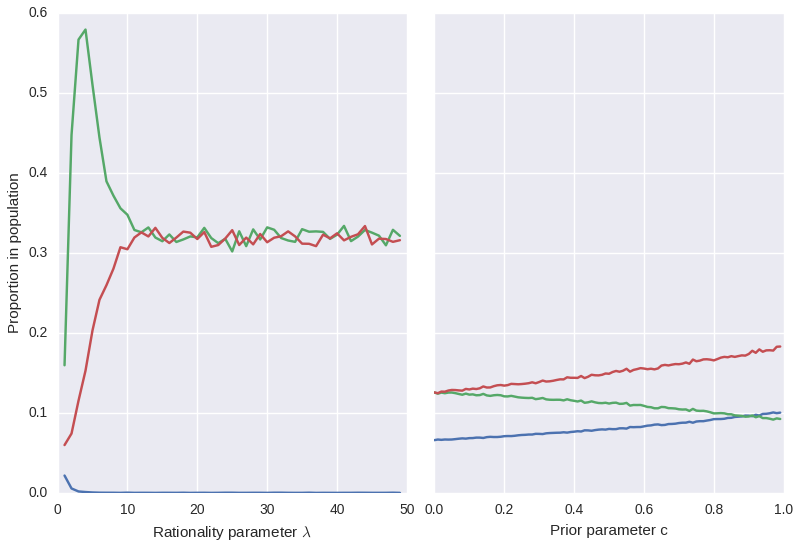
\includegraphics[width=\linewidth,height=\textheight,keepaspectratio]{./only-R-or-M}
\end{figure}
%
%\begin{figure}
%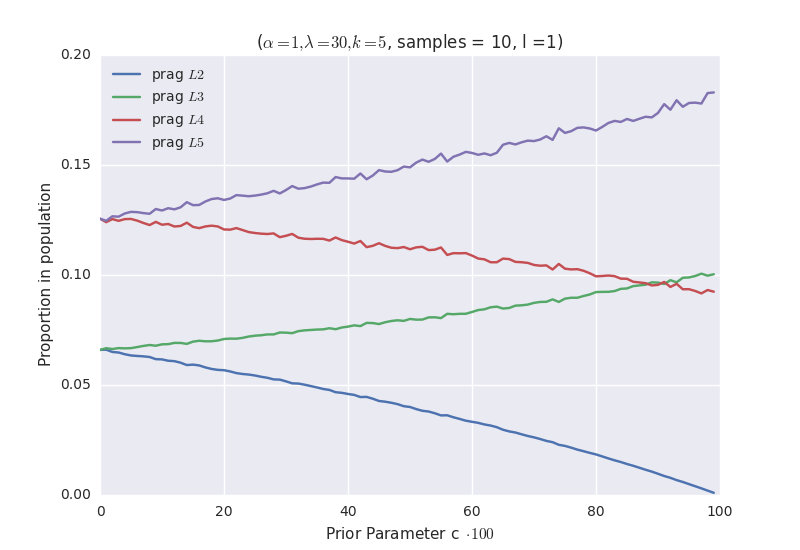
\includegraphics[width=\linewidth,height=\textheight,keepaspectratio]{../presentations/07learning}
%\end{figure}

\begin{figure}
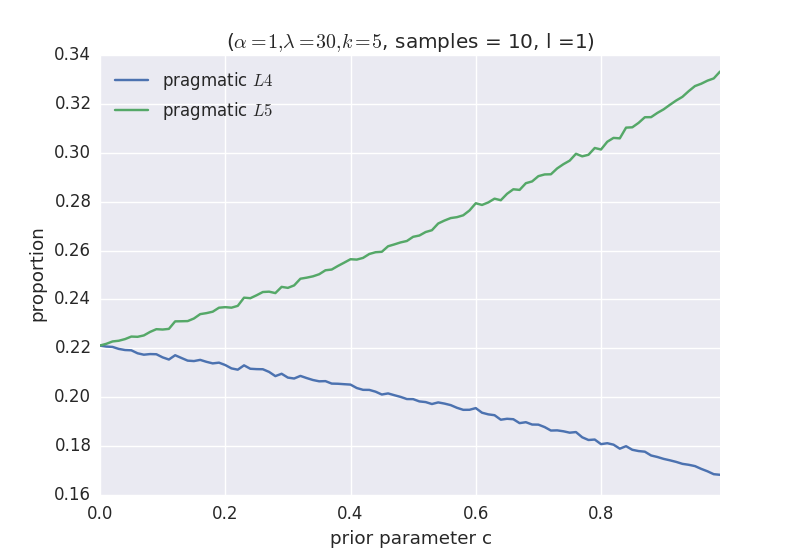
\includegraphics[width=\linewidth,height=\textheight,keepaspectratio]{../presentations/03cost-with-l1}
\end{figure}

\begin{figure}
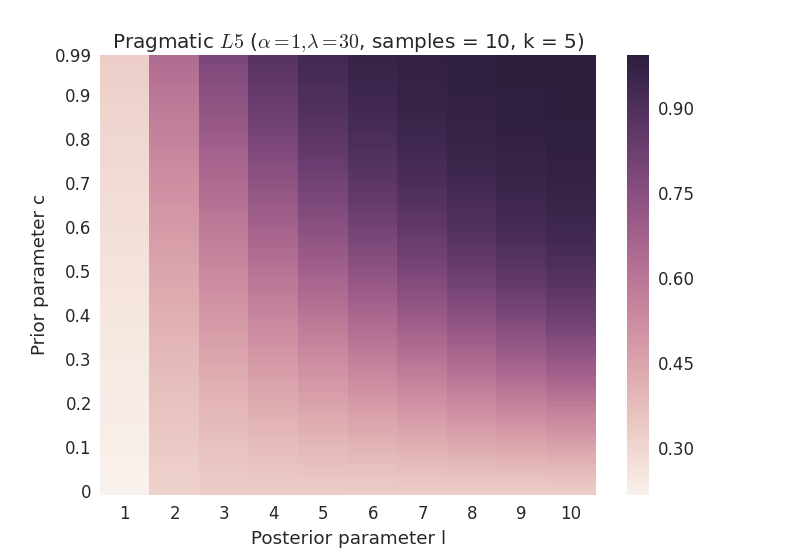
\includegraphics[width=\linewidth,height=\textheight,keepaspectratio]{../presentations/01heatmap}
\end{figure}

\section{Discussion}

\section{Extensions}
\subparagraph{(I) Cost for pragmatic reasoning.} At least in the CogSci setup the effect of adding cost to pragmatic reasoning is unsurprising: High cost for pragmatic signaling lowers the prevalence of pragmatic types. Lexica that semantically encode an upper-bound benefit the most from this. However, the cost needed to be substantial to make the pragmatic English-like lexicon stop being the incumbent type (particularly when learning is communal). 

\subparagraph{(II) Negative learning bias.} Instead of penalizing complex semantics (semantic upper-bounds) one may consider penalizing simple semantics (no upper-bounds). This is useful as a sanity check but also yields unsurprising results in the CogSci setup: The more learners are biased against simple semantics, the more prevalent are lexica that semantically encode upper-bounds. 

\subparagraph{(III) Inductive bias.} A second learning bias that codifies the idea that lexica should be uniform, i.e. be biased towards either lexicalizing an upper-bound for all weaker alternatives in a scalar pair or for none.

\subparagraph{(IV)  Uncertainty.} The other advantage of non-upper bounded semantics lies in being non-committal to the negation of stronger alternatives when the speaker is uncertain. Adding this to the model requires the most changes to our present setup and some additional assumptions about the cues available to players to discern the speaker's knowledge about the state she is in. 

\subparagraph{(V) More scalar pairs.} Taking into consideration more than one scalar pair. Preliminary results suggest that this does not influence the results in any meaningful way without further additions, e.g. by (III).

\subparagraph{(VI) More lexica.} Not necessary. Preliminary results suggest that considering more lexica has no noteworthy effect on the dynamics (tested with all possible 2x2 lexica).

\subparagraph{(VII) State frequencies.} Variations on state frequencies. This may have an interesting interaction with (III).

\subparagraph{(VIII) Reintroduction of communal learning.} One possibility: The probably $N_{ij}$ with which a child of $t_i$ adopts $t_j$ could be the weighted sum of $Q_{ij}$ (as before) and a vector we get from learning from all of the population: $L_j = \sum_d P(d | \vec{p})  P(t_j | d)$, where $P(d | \vec{p}) = \sum_{i} P(d | t_i)  \vec{p}_i$ is the probability of observing $d$ when learning from a random member of the present population distribution.

\section{Conclusion}

%%% Old snippets %%%
%\section{Conveying upper-bounds}
%Scalar inferences refer to the pragmatic derivation of an upper-bound for weak scalar expressions to the effect that stronger alternatives are inferred to not hold, e.g. {\em some students came} may be taken to convey that {\em not all students came}. The order of an expression such as {\em some} with respect to an alternative, e.g., {\em all}, is induced by entailment. For instance, {\em all students came} entails {\em most students came}, which in turn entails {\em some students came}. In this sense, {\em some} is weaker than {\em all}. A considerable class of natural language expressions do not lexicalize an upper-bound and can be ordered in this fashion, allowing for their pragmatic strengthening. As alluded at above, examples in English include numerals, scalar adjectives, quantifiers, modals, and connectives. \hl{possibly add some typological data on universality, frequency, monomorphemic status}
%
%The pragmatic enrichment of the semantic content of such expressions is enabled by mutual reasoning \citep{grice:1975}. More specifically, it is driven by interlocutors' mutual expectations of rational language use. The hearer reasons about the speaker's choice of a weak alternative over a stronger one. Had the speaker known that a stronger alternatives holds, she would have said so as this would have been more informative. Since she did not, the hearer can infer that the stronger alternative does not hold. Analogously, a speaker who reasons about her addressee may rely on her to derive this inference. In this way, a strengthened, upper-bounded, state of affairs can be conveyed without codifying the bound explicitly in the semantics.
%
%However, while pragmatics offers means to convey upper-bounds, the question why they are not part of the lexical meaning of these expressions remains. There are two main explanatory venues for this pattern. The first targets the functional advantages a lack of upper-bounds may confer to language users, whereas the second focuses on a learnability advantage of simpler over more complex semantic representations. 
%
%\paragraph{Function-based explanations.} Two assumptions are key to the pragmatic strengthening of weak alternatives: (the assumption of) cooperation and knowledge about the issue at hand. That is, the hearer needs to assume the speaker to be as informative as possible, i.e., not to withhold information, and that the speaker is knowlegeable, e.g., she knows whether {\em all students came}. Conversely, the speaker needs to assume the hearer to regard these conditions as satisfied. It is not difficult to imagine scenarios where either or both of these conditions are not given. For instance, the speaker may (be assumed to) not want to disclose all information about the students' attendance, or may have left early without being able to verify the attendance to a satisfactory degree. 
%
%\hl{Discussion of functional pressures for a lack of upper-bounds}

%\paragraph{Learning-based explanations.}
%
%\hl{Discussion of our main assumption that a lack of upper-bounds provides a learnability advantage framed in terms of relative representational simplicity over the codification of an upper-bound. {\bf Should this be made precise? If so, in which way?}}

%\bibliographystyle{apacite}
\bibliographystyle{unsrtnat}

%\setlength{\bibleftmargin}{.125in}
%\setlength{\bibindent}{-\bibleftmargin}
\bibliography{./bounds-rmd}


\end{document}
